% Options for packages loaded elsewhere
\PassOptionsToPackage{unicode}{hyperref}
\PassOptionsToPackage{hyphens}{url}
\PassOptionsToPackage{dvipsnames,svgnames*,x11names*}{xcolor}
%
\documentclass[
]{article}
\usepackage{amsmath,amssymb}
\usepackage{lmodern}
\usepackage{iftex}
\ifPDFTeX
  \usepackage[T1]{fontenc}
  \usepackage[utf8]{inputenc}
  \usepackage{textcomp} % provide euro and other symbols
\else % if luatex or xetex
  \usepackage{unicode-math}
  \defaultfontfeatures{Scale=MatchLowercase}
  \defaultfontfeatures[\rmfamily]{Ligatures=TeX,Scale=1}
\fi
% Use upquote if available, for straight quotes in verbatim environments
\IfFileExists{upquote.sty}{\usepackage{upquote}}{}
\IfFileExists{microtype.sty}{% use microtype if available
  \usepackage[]{microtype}
  \UseMicrotypeSet[protrusion]{basicmath} % disable protrusion for tt fonts
}{}
\makeatletter
\@ifundefined{KOMAClassName}{% if non-KOMA class
  \IfFileExists{parskip.sty}{%
    \usepackage{parskip}
  }{% else
    \setlength{\parindent}{0pt}
    \setlength{\parskip}{6pt plus 2pt minus 1pt}}
}{% if KOMA class
  \KOMAoptions{parskip=half}}
\makeatother
\usepackage{xcolor}
\IfFileExists{xurl.sty}{\usepackage{xurl}}{} % add URL line breaks if available
\IfFileExists{bookmark.sty}{\usepackage{bookmark}}{\usepackage{hyperref}}
\hypersetup{
  pdftitle={Quailty Improvement---Improved with R},
  pdfauthor={Mara Alexeev, MD, MPH1},
  colorlinks=true,
  linkcolor={Maroon},
  filecolor={Maroon},
  citecolor={Blue},
  urlcolor={blue},
  pdfcreator={LaTeX via pandoc}}
\urlstyle{same} % disable monospaced font for URLs
\usepackage[margin=1in]{geometry}
\usepackage{longtable,booktabs,array}
\usepackage{calc} % for calculating minipage widths
% Correct order of tables after \paragraph or \subparagraph
\usepackage{etoolbox}
\makeatletter
\patchcmd\longtable{\par}{\if@noskipsec\mbox{}\fi\par}{}{}
\makeatother
% Allow footnotes in longtable head/foot
\IfFileExists{footnotehyper.sty}{\usepackage{footnotehyper}}{\usepackage{footnote}}
\makesavenoteenv{longtable}
\usepackage{graphicx}
\makeatletter
\def\maxwidth{\ifdim\Gin@nat@width>\linewidth\linewidth\else\Gin@nat@width\fi}
\def\maxheight{\ifdim\Gin@nat@height>\textheight\textheight\else\Gin@nat@height\fi}
\makeatother
% Scale images if necessary, so that they will not overflow the page
% margins by default, and it is still possible to overwrite the defaults
% using explicit options in \includegraphics[width, height, ...]{}
\setkeys{Gin}{width=\maxwidth,height=\maxheight,keepaspectratio}
% Set default figure placement to htbp
\makeatletter
\def\fps@figure{htbp}
\makeatother
\setlength{\emergencystretch}{3em} % prevent overfull lines
\providecommand{\tightlist}{%
  \setlength{\itemsep}{0pt}\setlength{\parskip}{0pt}}
\setcounter{secnumdepth}{-\maxdimen} % remove section numbering
\usepackage{booktabs}
\usepackage{longtable}
\usepackage{array}
\usepackage{multirow}
\usepackage{wrapfig}
\usepackage{float}
\usepackage{colortbl}
\usepackage{pdflscape}
\usepackage{tabu}
\usepackage{threeparttable}
\usepackage{threeparttablex}
\usepackage[normalem]{ulem}
\usepackage{makecell}
\usepackage{xcolor}
\ifLuaTeX
  \usepackage{selnolig}  % disable illegal ligatures
\fi
\newlength{\cslhangindent}
\setlength{\cslhangindent}{1.5em}
\newlength{\csllabelwidth}
\setlength{\csllabelwidth}{3em}
\newenvironment{CSLReferences}[2] % #1 hanging-ident, #2 entry spacing
 {% don't indent paragraphs
  \setlength{\parindent}{0pt}
  % turn on hanging indent if param 1 is 1
  \ifodd #1 \everypar{\setlength{\hangindent}{\cslhangindent}}\ignorespaces\fi
  % set entry spacing
  \ifnum #2 > 0
  \setlength{\parskip}{#2\baselineskip}
  \fi
 }%
 {}
\usepackage{calc}
\newcommand{\CSLBlock}[1]{#1\hfill\break}
\newcommand{\CSLLeftMargin}[1]{\parbox[t]{\csllabelwidth}{#1}}
\newcommand{\CSLRightInline}[1]{\parbox[t]{\linewidth - \csllabelwidth}{#1}\break}
\newcommand{\CSLIndent}[1]{\hspace{\cslhangindent}#1}

\title{Quailty Improvement---Improved with R}
\author{Mara Alexeev, MD, MPH\textsuperscript{1}}
\date{}

\begin{document}
\maketitle

\textsuperscript{1} Boston Children's Hospital, Boston, MA, USA

Suggested length of workshop is \textbf{2 hours}.

\hypertarget{what-might-the-attendee-be-able-to-do-after-being-in-your-session}{%
\subsection{What might the attendee be able to do after being in your session?}\label{what-might-the-attendee-be-able-to-do-after-being-in-your-session}}

In this workshop, attendees will learn how to use R\textsuperscript{\protect\hyperlink{ref-R-base}{1}} to create, analyze, share, and publish the results of quality improvement (QI) projects based on tools\textsuperscript{\protect\hyperlink{ref-noauthor_quality_2017}{2}} published by the Institute for Healthcare Improvement and publishing recommendations from the Journal Of Graduate Medical Education.\textsuperscript{\protect\hyperlink{ref-wong_how_2016}{3}} This is a plug and play format that allows clinicians to directly create, analyze, and beautifully display their project and results with only a beginner's knowledge of R, R Markdown,\textsuperscript{\protect\hyperlink{ref-R-rmarkdown}{4}} and spreadsheets.

\hypertarget{description-of-the-problem-or-gap}{%
\subsection{Description of the problem or gap}\label{description-of-the-problem-or-gap}}

Many clinical informaticians participate in QI projects as either project leads or in supporting roles---helping other clinicians collect data from EHRs or implement projects within an EHR. There are many tools and guidelines for QI projects, but the tools are not well integrated into a single, comprehensive workflow of a QI project.

\hypertarget{conclusion}{%
\subsection{Conclusion}\label{conclusion}}

At the end of the workshop, participants will have the knowledge and materials to create a QI project write-up and analysis all within a single R Markdown file. They will learn how to customize the project to suit many QI project proposals. This simplification of the QI project workflow will allow attendees to more quickly prepare QI project proposals and analyze their results. More advanced knowledge of R packages discussed at the workshop will allow users to create highly customized presentations of their work.
A standardized tool to create QI projects will eliminate duplicated efforts in project workflows and allow results to be more quickly disseminated within an institution, posted online, or published in a journal.

\hypertarget{attendees-take-away-tool}{%
\subsection{Attendee's Take-away Tool}\label{attendees-take-away-tool}}

Attendee's will be able to access the QI tools through a publicly available GitHub repository, which they will be able to download and modify for their own purposes. They will also receive a curated selection of advanced resources for further learning.

\hypertarget{prerequisities}{%
\subsection{Prerequisities}\label{prerequisities}}

\begin{itemize}
\tightlist
\item
  Computer with internet connection
\item
  \href{https://support.rstudio.com/hc/en-us/articles/227449447-Supported-browsers-for-RStudio-Connect}{Supported browser}
\item
  RStudio Cloud account---\emph{free}
\item
  Review \href{https://commonmark.org/help/tutorial/}{preparatory materials} to learn Markdown basics---\emph{optional, but useful}
\end{itemize}

\hypertarget{level-of-content}{%
\subsection{Level of content}\label{level-of-content}}

All content will be accessible to a beginner R user. However, each section of the \textbf{Play} part of the workshop will have intermediate and advanced topics embedded in the code for more advanced users to manipulate.

\hypertarget{instructors-experience-teaching-similar-content}{%
\subsection{Instructor's experience teaching similar content}\label{instructors-experience-teaching-similar-content}}

Mara Alexeev is a pediatrician and clinical informatics fellow. She is also a graduate student working on her Masters in Biomedical Informatics at Harvard Medical School. She was part of the organizing committee for the 2020 R/Medicine conference and is a co-organizer for R-Ladies Boston, where she recently hosted a workshop on how to make and maintain a CV in R.

\hypertarget{outline-of-topics}{%
\subsection{Outline of topics}\label{outline-of-topics}}

\textbf{Systems check} \emph{\textasciitilde15 minutes}

\begin{itemize}
\tightlist
\item
  Confirm accounts set up
\item
  Discuss pre-workshop materials
\end{itemize}

\textbf{Introduction} \emph{\textasciitilde30 minutes}

\begin{itemize}
\tightlist
\item
  R Markdown demo
\item
  Knit a document
\item
  View a demo GitHub Page
\end{itemize}

\textbf{Play} \emph{\textasciitilde30 minutes}

\begin{itemize}
\tightlist
\item
  Modify cause and effect diagrams within R
\item
  Customize tables and graphs for a Failure Modes and Effects Analysis (FMEA) and a Pareto Chart
\item
  Learn how to make scatter plots (Figure \ref{fig:scatter}) and histograms (Figure \ref{fig:histo}) with ggplot2
\item
  Create runcharts that can update as data is collected with a click of button
\item
  Use the automated bibliographic capabilities of R
\end{itemize}

\textbf{Wrap Up and Discussion} \emph{\textasciitilde20 minutes}

\begin{itemize}
\tightlist
\item
  Discussion of participants questions
\item
  Watch demonstration of publishing to Github Page
\item
  Preview of advanced materials
\end{itemize}

\begin{figure}

{\centering 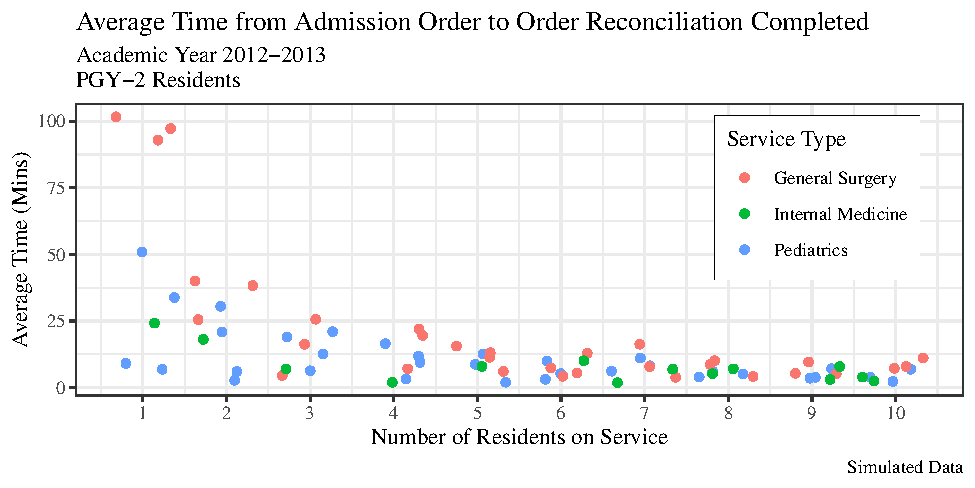
\includegraphics{qi_workshop_files/figure-latex/scatter-1} 

}

\caption{Example scatter plot made in R}\label{fig:scatter}
\end{figure}

\begin{figure}

{\centering 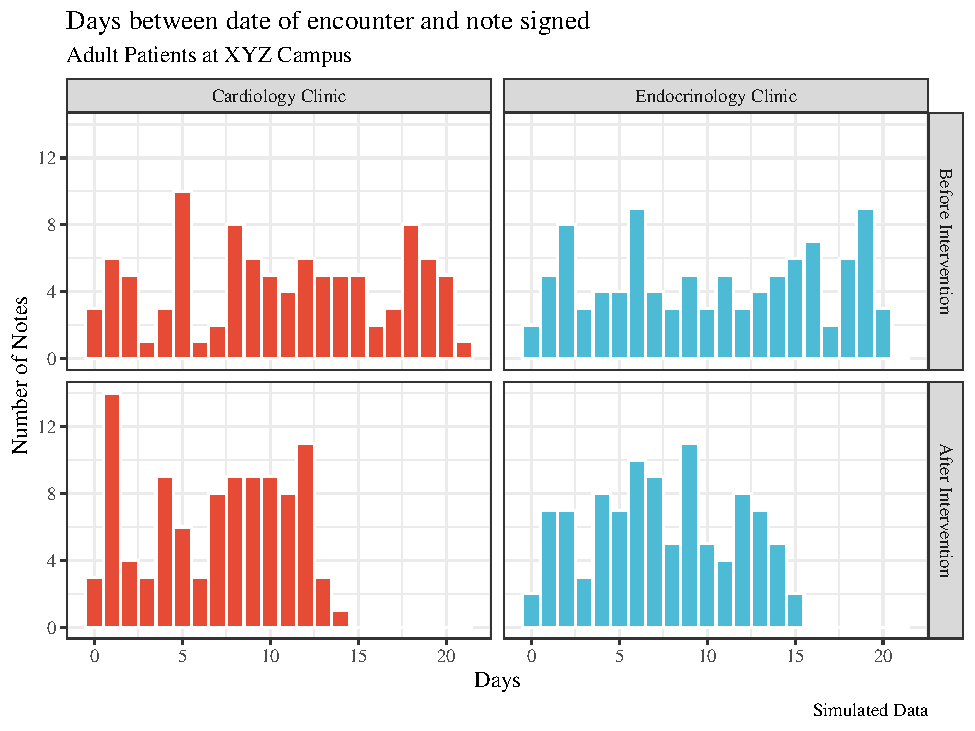
\includegraphics{qi_workshop_files/figure-latex/histo-1} 

}

\caption{Example histogram created in R}\label{fig:histo}
\end{figure}

\hypertarget{use-of-knowledge-acquired-at-previous-amia-events}{%
\subsection{Use of Knowledge Acquired at Previous AMIA Events}\label{use-of-knowledge-acquired-at-previous-amia-events}}

No.~

\hypertarget{references}{%
\subsection*{References}\label{references}}
\addcontentsline{toc}{subsection}{References}

\hypertarget{refs}{}
\begin{CSLReferences}{0}{0}
\leavevmode\vadjust pre{\hypertarget{ref-R-base}{}}%
1. R Core Team. R: A language and environment for statistical computing {[}Internet{]}. Vienna, Austria: R Foundation for Statistical Computing; 2020. Available from: \url{https://www.R-project.org/}

\leavevmode\vadjust pre{\hypertarget{ref-noauthor_quality_2017}{}}%
2. Quality {Improvement} {Essentials} {Toolkit} {[}Internet{]}. 2017 ;{[}cited 2021 Jan. 13{]} Available from: \url{http://www.ihi.org/resources/_layouts/download.aspx?SourceURL=\%2fresources\%2fKnowledge+Center+Assets\%2fTools+-+QualityImprovementEssentialsToolkit_e14261f9-05ff-4a7b-ba25-58c85c4c9e9a\%2fQIEssentialsToolkit.pdf}

\leavevmode\vadjust pre{\hypertarget{ref-wong_how_2016}{}}%
3. Wong BM, Sullivan GM. How to {Write} {Up} {Your} {Quality} {Improvement} {Initiatives} for {Publication} {[}Internet{]}. Journal of Graduate Medical Education. 2016 May ;8(2):128--133.{[}cited 2021 Jan. 12{]} Available from: \url{https://www.ncbi.nlm.nih.gov/pmc/articles/PMC4857497/}

\leavevmode\vadjust pre{\hypertarget{ref-R-rmarkdown}{}}%
4. Allaire J, Xie Y, McPherson J, Luraschi J, Ushey K, Atkins A, Wickham H, Cheng J, Chang W, Iannone R. Rmarkdown: Dynamic documents for r {[}Internet{]}. 2021. Available from: \url{https://CRAN.R-project.org/package=rmarkdown}

\end{CSLReferences}

\end{document}
